\section{General Optimization Methods}

    \begin{frame}{General Optimization Methods}
        \centering
        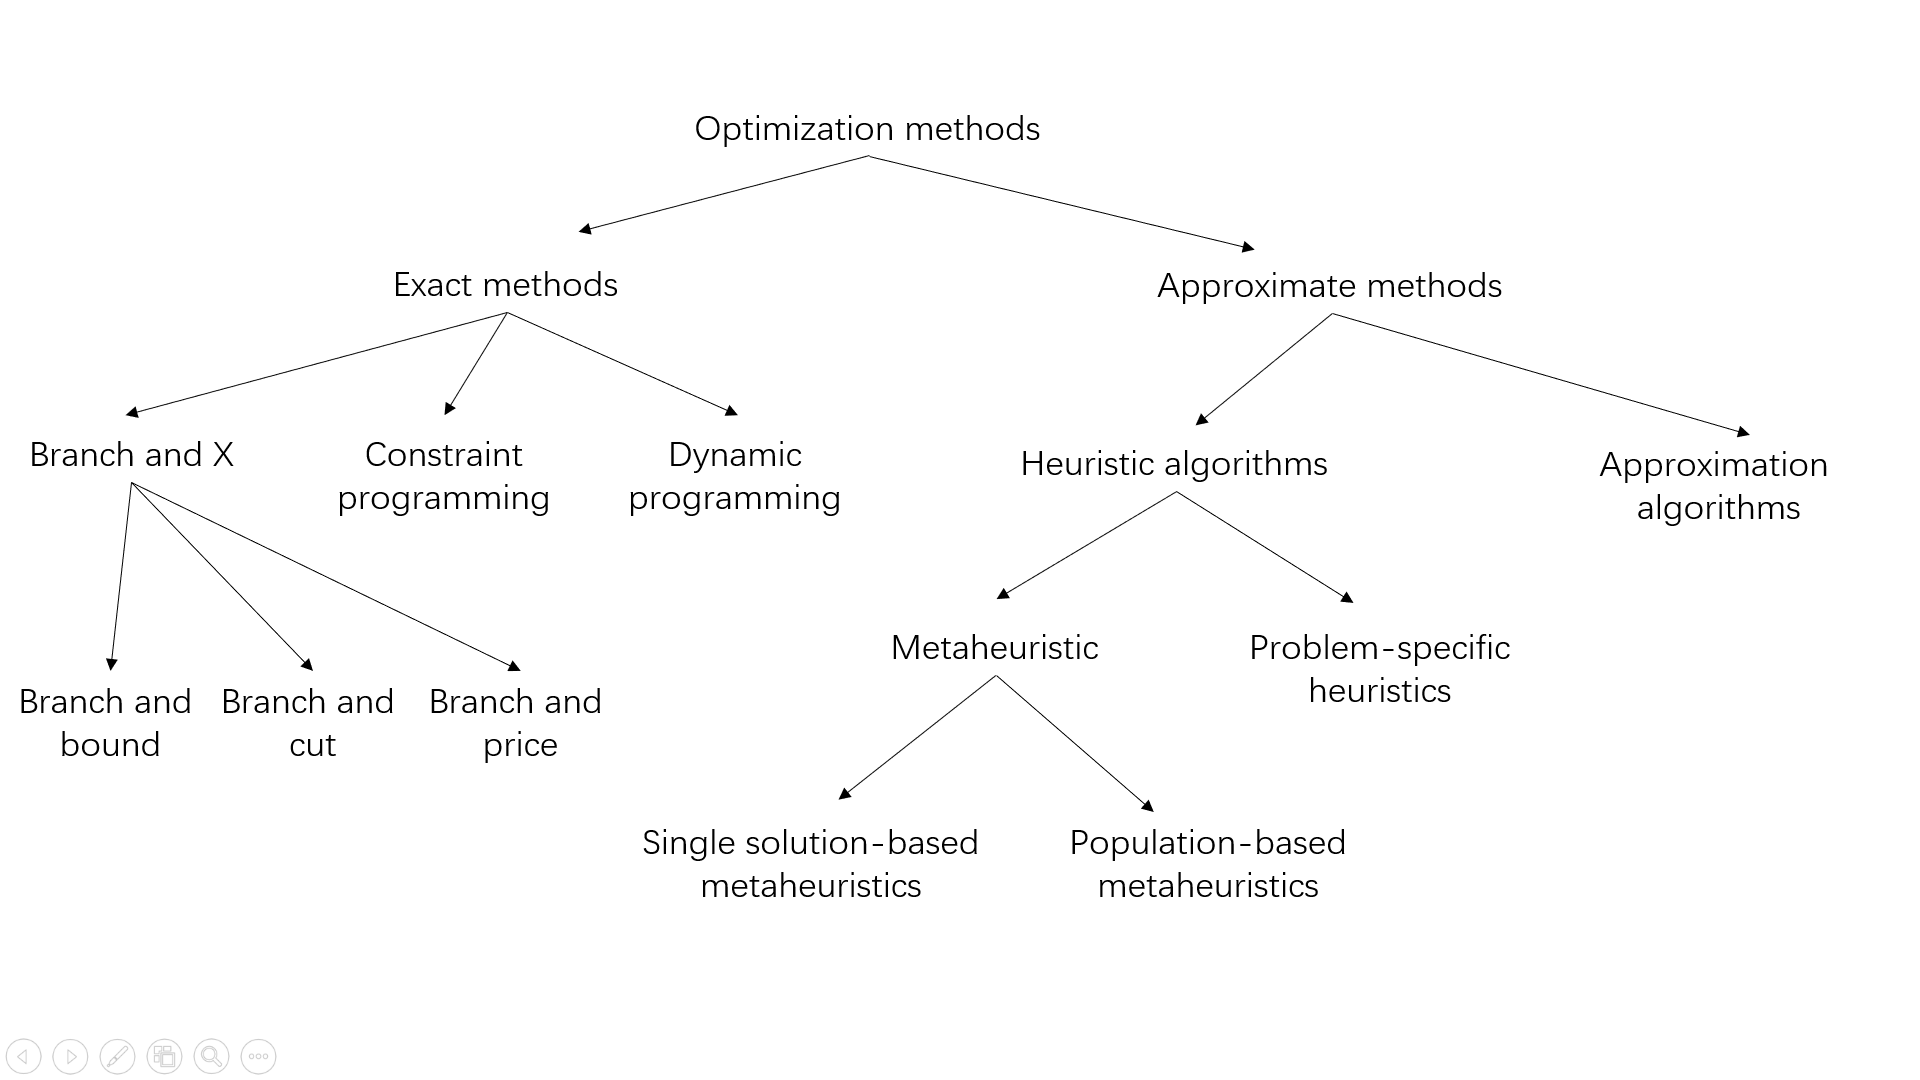
\includegraphics[width = 1\textwidth]{images/opt.png}
    \end{frame}

    \subsection{Exact Methods}
    \frame{\sectionpage}

    \begin{frame}{Exact Methods}
      \Large
      \begin{spacing}{2}
        \begin{itemize}
          \item<+-> Branch and X
            \begin{enumerate}
            \item<+>  Branch and bound
            \item<+>  Branch and cut
            \item<+>  Branch and price
            \end{enumerate}
        \end{itemize}
      \end{spacing}
    \end{frame}

    \begin{frame}{Branch and bound}
      \centering
      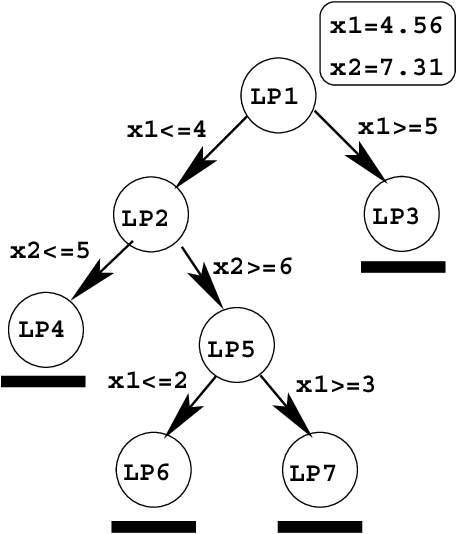
\includegraphics[width = 0.55\textwidth]{images/Branch.png}
    \end{frame}

    \begin{frame}{Cutting Plane Method}
      \centering
      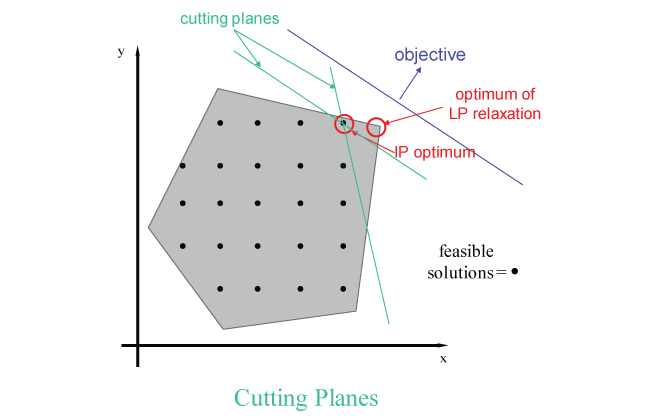
\includegraphics[width = 1\textwidth]{images/CP.png}
    \end{frame}

    \begin{frame}{Gomory's Cut}
      \begin{itemize}

      \item Using the simplex method:
      $x_{i}+\sum{\bar {a}}_{i,j}x_{j}={\bar {b}}_{i}$ \\

      where $x_i$ are the basic variables and the $x_j$'s are the nonbasic variables.

      \item Rewrite this equation: integer parts(left) and the fractional parts(right):

      $x_{i}+\sum \lfloor {\bar {a}}_{i,j}\rfloor x_{j}-\lfloor {\bar {b}}_{i}\rfloor ={\bar {b}}_{i}-\lfloor {\bar {b}}_{i}\rfloor -\sum ({\bar {a}}_{i,j}-\lfloor {\bar {a}}_{i,j}\rfloor )x_{j}.$ \\

      \item Right side is less than 1 and the left side is an integer, therefore the inequality:
      \textcolor{red}{${\bar {b}}_{i}-\lfloor {\bar {b}}_{i}\rfloor -\sum ({\bar {a}}_{i,j}-\lfloor {\bar {a}}_{i,j}\rfloor )x_{j}\leq 0 $}
      must hold for any integer point in the feasible region.

      \item The inequality above is a cut with the desired properties. Introducing a new slack variable $x_k$ for this inequality, a new constraint is added to the linear program, namely

      \textcolor{red}{$x_{k}+\sum (\lfloor {\bar {a}}_{i,j}\rfloor -{\bar {a}}_{i,j})x_{j}=\lfloor {\bar {b}}_{i}\rfloor -{\bar {b}}_{i},\,x_{k}\geq 0,\,x_{k}{\mbox{ an integer}}$.}
      \end{itemize}
    \end{frame}

    \begin{frame}{Branch and price}
      \centering
      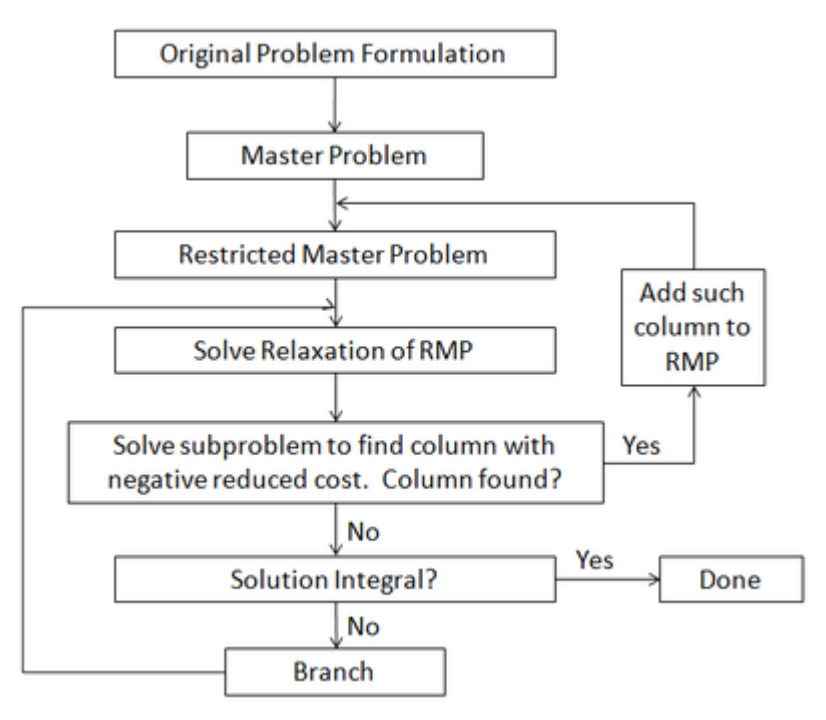
\includegraphics[width = 0.7\textwidth]{images/branch_price.png}
    \end{frame}

    \begin{frame}{Exact Methods}
      \Large
      \begin{spacing}{1.5}
        \begin{itemize}
          \item Branch and X
          \item<+-> Dynamic programming
          \item<+-> Constraint programming
          \item<+-> Enumeration method
        \end{itemize}
      \end{spacing}
    \end{frame}



    \subsection{Approximate Methods}
    \frame{\sectionpage}

    \begin{frame}{Approximate Methods}
      \Large
      \begin{itemize}
        \item Heuristic algorithms
        \vspace{4pt}
        \begin{enumerate}
          \item<+->  Metaheuristic
            \begin{enumerate}
              \item<+>[*] Single solution-based metaheuristics
              \item<+>[*] Population-based metaheuristics
            \end{enumerate}
          \vspace{4pt}
          \item<+->  Problem-specific heuristics
        \end{enumerate}
        \item<+-> Approximate algorithms
      \end{itemize}
    \end{frame}

    \begin{frame}{Single solution-based metaheuristics}
      \Large
      \begin{spacing}{2}
        \begin{itemize}
          \item Simulated Annealing Algorithm
          \item Tabu Search
          \item Variable Neighborhood Search
          \item Adaptive Large Neighborhood Search
        \end{itemize}
      \end{spacing}
    \end{frame}

    \begin{frame}{Population-based heuristics}
      \Large
      \begin{spacing}{2}
        \begin{itemize}
          \item Genetic Algorithm
          \item Ant Colony Optimization
          \item Partical Swarm Optimization
        \end{itemize}
      \end{spacing}

    \end{frame}

    % Using the simplex method to solve a linear program produces a set of equations of the form
    % $x_{i}+\sum{\bar {a}}_{i,j}x_{j}={\bar {b}}_{i}$ \\
    %
    % where xi is a basic variable and the xj's are the nonbasic variables. Rewrite this equation so that the integer parts are on the left side and the fractional parts are on the right side:
    %
    % $x_{i}+\sum \lfloor {\bar {a}}_{i,j}\rfloor x_{j}-\lfloor {\bar {b}}_{i}\rfloor ={\bar {b}}_{i}-\lfloor {\bar {b}}_{i}\rfloor -\sum ({\bar {a}}_{i,j}-\lfloor {\bar {a}}_{i,j}\rfloor )x_{j}.$ \\
    %
    % For any integer point in the feasible region the right side of this equation is less than 1 and the left side is an integer, therefore the common value must be less than or equal to 0. So the inequality
    %
    % $ {\bar {b}}_{i}-\lfloor {\bar {b}}_{i}\rfloor -\sum ({\bar {a}}_{i,j}-\lfloor {\bar {a}}_{i,j}\rfloor )x_{j}\leq 0 $
    %
    % must hold for any integer point in the feasible region. Furthermore, nonbasic variables are equal to 0s in any basic solution and if xi is not an integer for the basic solution x,
    %
    % $ {\bar {b}}_{i}-\lfloor {\bar {b}}_{i}\rfloor -\sum ({\bar {a}}_{i,j}-\lfloor {\bar {a}}_{i,j}\rfloor )x_{j}={\bar {b}}_{i}-\lfloor {\bar {b}}_{i}\rfloor >0. $
    %
    % So the inequality above excludes the basic feasible solution and thus is a cut with the desired properties. Introducing a new slack variable xk for this inequality, a new constraint is added to the linear program, namely
    %
    % $ x_{k}+\sum (\lfloor {\bar {a}}_{i,j}\rfloor -{\bar {a}}_{i,j})x_{j}=\lfloor {\bar {b}}_{i}\rfloor -{\bar {b}}_{i},\,x_{k}\geq 0,\,x_{k}{\mbox{ an integer}}. $
